\section{Fehler und Ausnahmen}

\begin{frame}[fragile]
\frametitle{Syntax Errors, Indentation Errors}
Fehler beim Parsen: \alert{Programm wird nicht ausgef"uhrt}. Z.B.: 
\begin{itemize}
\item Klammerungsfehler
\item Falsche oder fehlende Semikolons, Doppelpunkte, Kommas
\item Einr"uckungsfehler
\end{itemize}
\begin{lstlisting}[style=Python]
print "Ich laufe..."
def add(a, b)
   return a + b
\end{lstlisting}
\begin{lstlisting}[style=Shell]
$ ./addiere.py
  File "addiere.py", line 1
    def add(a, b)
                ^
SyntaxError: invalid syntax
\end{lstlisting}
\end{frame}

\begin{frame}[fragile]
\frametitle{Ausnahmen}
Ausnahmen (Exceptions) treten \alert{zur Laufzeit} auf:
\begin{lstlisting}[style=Python]
import math
print "Ich laufe..."
math.foo()
\end{lstlisting}
\begin{lstlisting}[style=Shell]
$ ./test.py
Ich laufe...
Traceback (most recent call last):
  File "test.py", line 3, in ?
    math.foo()
AttributeError: 'module' object has no 
attribute 'foo'
\end{lstlisting}
\end{frame}

\begin{frame}[fragile]
\frametitle{Ausnahmen behandeln}
\begin{lstlisting}[style=Python]
try:
    s = raw_input("Gib eine Zahl ein: ")
    zahl = float(s)
except ValueError:
    print "Das ist keine Zahl!"
\end{lstlisting}
\begin{itemize}
\item \texttt{except}-Block wird ausgef"uhrt, wenn Code im \texttt{try}-Block eine passende Ausnahme wirft
\item danach l"auft Programm normal weiter
\item nicht behandelte Ausnahmen f"uhren zum Programmabbruch
\end{itemize}
Verschiedene Ausnahmen abfangen:
\begin{lstlisting}[style=Python]
except (ValueError, TypeError, NameError):
\end{lstlisting}
\end{frame}

\begin{frame}[fragile]
\frametitle{Ausnahmen behandeln}
\begin{lstlisting}[style=Python]
try:
    s = raw_input("Gib eine Zahl ein: ")
    zahl = 1/float(s)
except ValueError:
    print "Das ist keine Zahl!"
except ZeroDivisionError:
    print "Man kann nicht durch Null teilen!"
except:
    print "Was ist hier passiert?"
\end{lstlisting}
\begin{itemize}
\item Mehrere \texttt{except}-Statements f"ur verschiedene Ausnahmen
\item Letztes \texttt{except} kann ohne Ausnahme-Typ verwendet werden: F"angt alle verbleibenen Ausnahmen ab
\begin{itemize}
\item Vorsicht: Kann ungewollte Programmierfehler verdecken!
\end{itemize}
\end{itemize}
\end{frame}

\begin{frame}[fragile]
\frametitle{Ausnahmen behandeln}
\begin{itemize}
\item \alert{\texttt{else}} wird ausgef"uhrt, wenn keine Ausnahme auftrat
\item \alert{\texttt{finally}} wird in \alert{jedem} Fall ausgef"uhrt
\end{itemize}
\begin{lstlisting}[style=Python]
try:
    f = open("spam")
except IOError:
    print "Cannot open file"
else:
    print f.read()
    f.close()
finally:
    print "Ende von try."
\end{lstlisting}
\end{frame}

\begin{frame}[fragile]
\frametitle{Ausnahme-Objekte}
Auf das Ausnahme-Objekt zugreifen:
\begin{lstlisting}[style=Python]
try:
    f = open("spam")
except IOError, e:
    print e.errno, e.strerror
    print e
\end{lstlisting}
\begin{lstlisting}[style=Shell]
$ python test.py
2 No such file or directory
[Errno 2] No such file or directory: 'spam'
\end{lstlisting}%$
\end{frame}

\begin{frame}
\frametitle{Ausnahmen in Funktionsaufrufen}
\begin{figure}
\centering
\only<1>
{
  \begin{tikzpicture}
  \draw [black] (0, 0.2) node {draw()};
  \draw [white, ->] (0, 0) arc(180:270:15pt) node[anchor=west] {rectangle()};
  \draw [white, ->] (1.5, -0.7) arc(180:270:15pt) 
                    -- (2.5, -1.23) node[anchor=west] {line()};
  \draw [white] (4.6, -1.23) node {Exception!};
  \draw [white, ->] (4.5, -1.0) arc(0:90:15pt) -- (2.8, -0.47);
  \draw [white, ->] (2.6, -0.3) arc(0:90:15pt) -- (0.8, 0.225);
  \end{tikzpicture}
}

\only<2>
{
  \begin{tikzpicture}
  \draw [black] (0, 0.2) node {draw()};
  \draw [black, ->] (0, 0) arc(180:270:15pt) node[anchor=west] {rectangle()};
  \draw [white, ->] (1.5, -0.7) arc(180:270:15pt) 
                    -- (2.5, -1.23) node[anchor=west] {line()};
  \draw [white] (4.6, -1.23) node {Exception!};
  \draw [white, ->] (4.5, -1.0) arc(0:90:15pt) -- (2.8, -0.47);
  \draw [white, ->] (2.6, -0.3) arc(0:90:15pt) -- (0.8, 0.225);
  \end{tikzpicture}
}

\only<3>
{
  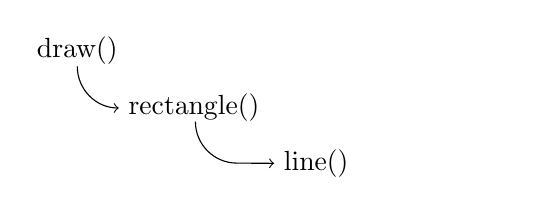
\begin{tikzpicture}
  \draw [black] (0, 0.2) node {draw()};
  \draw [black, ->] (0, 0) arc(180:270:15pt) node[anchor=west] {rectangle()};
  \draw [black, ->] (1.5, -0.7) arc(180:270:15pt) 
                    -- (2.5, -1.23) node[anchor=west] {line()};
  \draw [white] (4.6, -1.23) node {Exception!};
  \draw [white, ->] (4.5, -1.0) arc(0:90:15pt) -- (2.8, -0.47);
  \draw [white, ->] (2.6, -0.3) arc(0:90:15pt) -- (0.8, 0.225);
  \end{tikzpicture}
}

\only<4>
{
  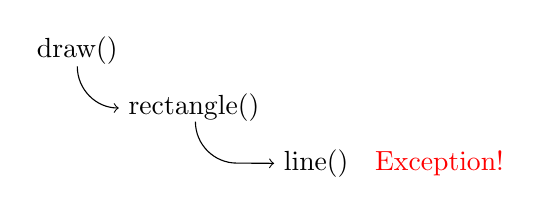
\begin{tikzpicture}
  \draw [black] (0, 0.2) node {draw()};
  \draw [black, ->] (0, 0) arc(180:270:15pt) node[anchor=west] {rectangle()};
  \draw [black, ->] (1.5, -0.7) arc(180:270:15pt) 
                    -- (2.5, -1.23) node[anchor=west] {line()};
  \draw [red] (4.6, -1.23) node {Exception!};
  \draw [white, ->] (4.5, -1.0) arc(0:90:15pt) -- (2.8, -0.47);
  \draw [white, ->] (2.6, -0.3) arc(0:90:15pt) -- (0.8, 0.225);
  \end{tikzpicture}
}

\only<5>
{
  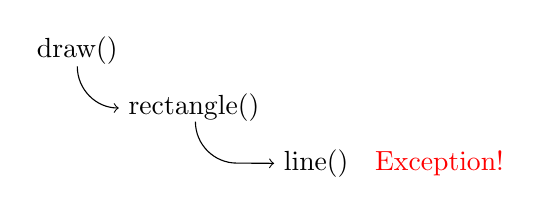
\begin{tikzpicture}
  \draw [black] (0, 0.2) node {draw()};
  \draw [black, ->] (0, 0) arc(180:270:15pt) node[anchor=west] {rectangle()};
  \draw [black, ->] (1.5, -0.7) arc(180:270:15pt) 
                    -- (2.5, -1.23) node[anchor=west] {line()};
  \draw [red] (4.6, -1.23) node {Exception!};
  \draw [white, ->] (4.5, -1.0) arc(0:90:15pt) -- (2.8, -0.47);
  \draw [white, ->] (2.6, -0.3) arc(0:90:15pt) -- (0.8, 0.225);
  \end{tikzpicture}
}

\only<6>
{
  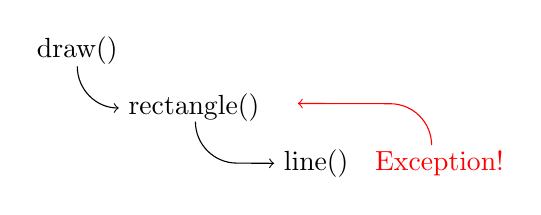
\begin{tikzpicture}
  \draw [black] (0, 0.2) node {draw()};
  \draw [black, ->] (0, 0) arc(180:270:15pt) node[anchor=west] {rectangle()};
  \draw [black, ->] (1.5, -0.7) arc(180:270:15pt) 
                    -- (2.5, -1.23) node[anchor=west] {line()};
  \draw [red] (4.6, -1.23) node {Exception!};
  \draw [red, ->] (4.5, -1.0) arc(0:90:15pt) -- (2.8, -0.47);
  \draw [white, ->] (2.6, -0.3) arc(0:90:15pt) -- (0.8, 0.225);
  \end{tikzpicture}
}

\only<7>
{
  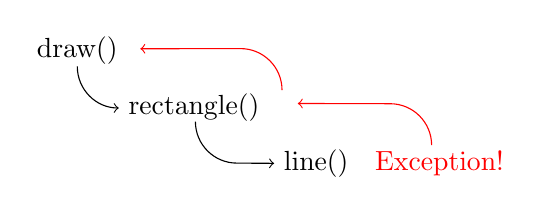
\begin{tikzpicture}
  \draw [black] (0, 0.2) node {draw()};
  \draw [black, ->] (0, 0) arc(180:270:15pt) node[anchor=west] {rectangle()};
  \draw [black, ->] (1.5, -0.7) arc(180:270:15pt) 
                    -- (2.5, -1.23) node[anchor=west] {line()};
  \draw [red] (4.6, -1.23) node {Exception!};
  \draw [red, ->] (4.5, -1.0) arc(0:90:15pt) -- (2.8, -0.47);
  \draw [red, ->] (2.6, -0.3) arc(0:90:15pt) -- (0.8, 0.225);
  \end{tikzpicture}
}
\end{figure}
\begin{itemize}
\item<1-> Funktion ruft Unterfunktionen auf.
\item<4-> Unterfunktion wirft Ausnahme.
\item<5-> Wird Ausnahme behandelt?
\item<6-> Nein: Gib Ausnahme an aufrufende Funktion weiter.
\end{itemize}
\end{frame}

\begin{frame}[fragile]
\frametitle{Ausnahmen ausl"osen}
Ausnahmen weiterreichen:
\begin{lstlisting}[style=Python]
try:
    f = open("spam")
except IOError:
    print "Fehler beim Oeffnen!"
    raise
\end{lstlisting}
\vspace{3mm}
Ausnahmen ausl"osen:
\begin{lstlisting}[style=Python]
def gauss_solver(matrix):
    # Wichtiger Code
    raise ValueError("Matrix singulaer")
\end{lstlisting}
\end{frame}

%%% Local Variables: 
%%% mode: latex
%%% latex-run-command: pdflatex
%%% TeX-master: "vortrag"
%%% End: 
